\documentclass{standalone}
\usepackage{tikz}
\usetikzlibrary{patterns}
\usetikzlibrary{positioning}
\usetikzlibrary{patterns, positioning}
\usetikzlibrary{shapes.misc}
\usepackage[outline]{contour}
\contourlength{1.5pt} 
\usetikzlibrary{calc}
        \usepackage{relsize}
        \tikzset{fontscale/.style = {font=\relsize{#1}}}

\begin{document}
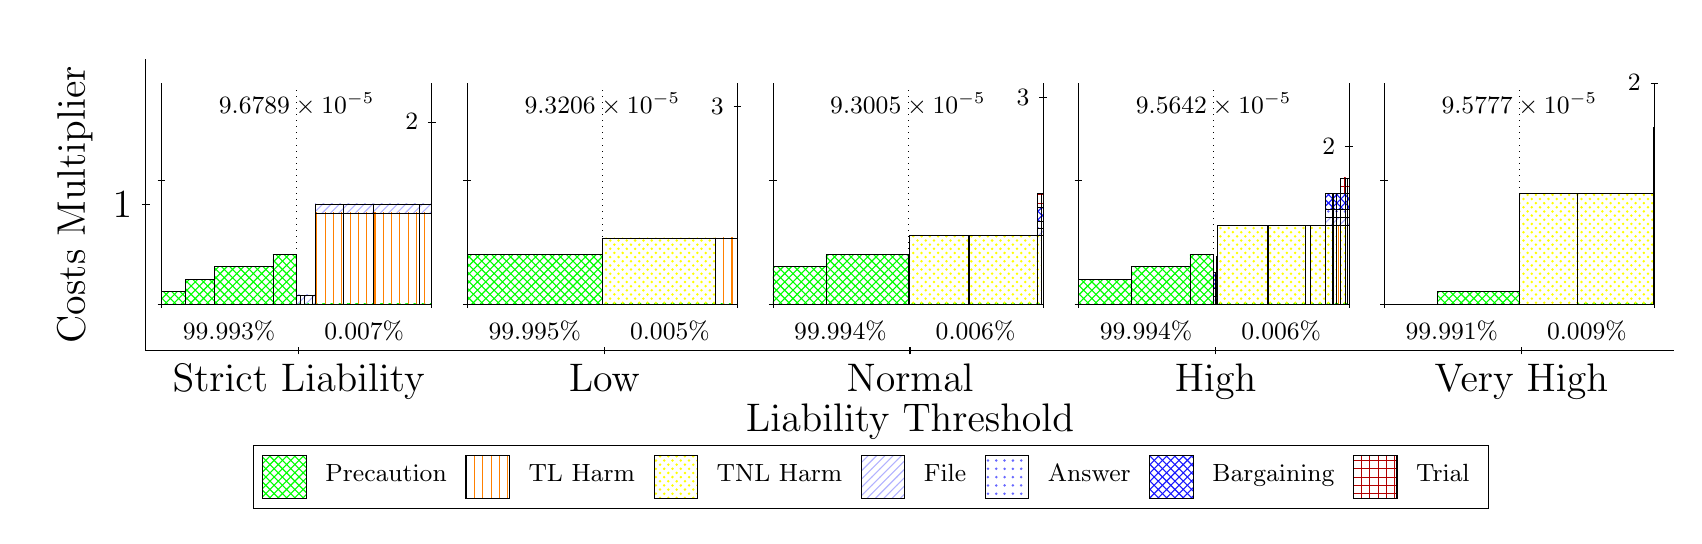
\begin{tikzpicture}
\clip(-0.5,-1.1) rectangle +(20.91,6.2);
\draw[black] (1,1) -- (1,4.7);
\node[rotate=90, fontscale=2, anchor=center] at (0.1, 2.85) {Costs Multiplier};
\draw[black] (0.95,2.85) -- (1.05,2.85);
\node[fontscale=2, anchor=east] at (0.95, 2.85) {1};

\draw[black] (1,1) -- (20.41,1);
\node[fontscale=2, anchor=center] at (10.705, 0.1) {Liability Threshold};
\draw[black] (2.941,0.95) -- (2.941,1.05);
\node[fontscale=2, anchor=north] at (2.941, 0.95) {Strict Liability};
\draw[black] (6.823,0.95) -- (6.823,1.05);
\node[fontscale=2, anchor=north] at (6.823, 0.95) {Low};
\draw[black] (10.705,0.95) -- (10.705,1.05);
\node[fontscale=2, anchor=north] at (10.705, 0.95) {Normal};
\draw[black] (14.587,0.95) -- (14.587,1.05);
\node[fontscale=2, anchor=north] at (14.587, 0.95) {High};
\draw[black] (18.469,0.95) -- (18.469,1.05);
\node[fontscale=2, anchor=north] at (18.469, 0.95) {Very High};


\draw[pattern=crosshatch, pattern color=green,draw=black,very thin] (1.2,1.592) rectangle (1.5023,1.7494);
\draw[pattern=crosshatch, pattern color=green,draw=black,very thin] (1.5023,1.592) rectangle (1.8725,1.9069);
\draw[pattern=crosshatch, pattern color=green,draw=black,very thin] (1.8725,1.592) rectangle (2.6136,2.0643);
\draw[pattern=crosshatch, pattern color=green,draw=black,very thin] (2.6136,1.592) rectangle (2.916,2.2218);
\draw[pattern=crosshatch, pattern color=green,draw=black,very thin] (2.916,1.592) rectangle (2.9572,1.592);
\draw[pattern=north east lines, pattern color=blue!30,draw=black,very thin] (2.916,1.592) rectangle (2.9572,1.7075);
\draw[pattern=crosshatch, pattern color=green,draw=black,very thin] (2.9572,1.592) rectangle (3.0077,1.592);
\draw[pattern=north east lines, pattern color=blue!30,draw=black,very thin] (2.9572,1.592) rectangle (3.0077,1.7075);
\draw[pattern=crosshatch, pattern color=green,draw=black,very thin] (3.0077,1.592) rectangle (3.1087,1.592);
\draw[pattern=north east lines, pattern color=blue!30,draw=black,very thin] (3.0077,1.592) rectangle (3.1087,1.7076);
\draw[pattern=crosshatch, pattern color=green,draw=black,very thin] (3.1087,1.592) rectangle (3.1499,1.592);
\draw[pattern=north east lines, pattern color=blue!30,draw=black,very thin] (3.1087,1.592) rectangle (3.1499,1.7076);
\draw[pattern=crosshatch, pattern color=green,draw=black,very thin] (3.1499,1.592) rectangle (3.5134,1.592);
\draw[pattern=vertical lines, pattern color=orange,draw=black,very thin] (3.1499,1.592) rectangle (3.5134,2.7472);
\draw[pattern=north east lines, pattern color=blue!30,draw=black,very thin] (3.1499,2.7472) rectangle (3.5134,2.8628);
\draw[pattern=crosshatch, pattern color=green,draw=black,very thin] (3.5134,1.592) rectangle (3.8947,1.592);
\draw[pattern=vertical lines, pattern color=orange,draw=black,very thin] (3.5134,1.592) rectangle (3.8947,2.7473);
\draw[pattern=north east lines, pattern color=blue!30,draw=black,very thin] (3.5134,2.7473) rectangle (3.8947,2.8628);
\draw[pattern=crosshatch, pattern color=green,draw=black,very thin] (3.8947,1.592) rectangle (4.4695,1.592);
\draw[pattern=vertical lines, pattern color=orange,draw=black,very thin] (3.8947,1.592) rectangle (4.4695,2.7473);
\draw[pattern=north east lines, pattern color=blue!30,draw=black,very thin] (3.8947,2.7473) rectangle (4.4695,2.8628);
\draw[pattern=crosshatch, pattern color=green,draw=black,very thin] (4.4695,1.592) rectangle (4.632,1.592);
\draw[pattern=vertical lines, pattern color=orange,draw=black,very thin] (4.4695,1.592) rectangle (4.632,2.7473);
\draw[pattern=north east lines, pattern color=blue!30,draw=black,very thin] (4.4695,2.7473) rectangle (4.632,2.8628);
\node[font=\small,text=black,anchor=north] at (2.916, 4.4) {$9.6789\times 10^{-5}$};
\draw[black,very thin] (1.2,1.592) -- (1.2,4.4);
\draw[black,very thin] (1.15,1.592) -- (1.25,1.592);
\node[font=\small,text=black, anchor=west] at (1.15, 1.592) {};
\draw[black,very thin] (1.15,3.1664) -- (1.25,3.1664);
\node[font=\small,text=black, anchor=west] at (1.15, 3.1664) {};

\draw[black,dotted,very thin] (2.916,1.6762) -- (2.916,4.3158);
\draw[black,very thin] (4.632,1.592) -- (4.632,4.4);
\draw[black,very thin] (4.582,3.9025) -- (4.682,3.9025);
\node[font=\small,text=black, anchor=east] at (4.582, 3.9025) {\contour{white}{2}};

\draw[black,very thin] (1.2,1.592) -- (4.632,1.592);
\draw[black,very thin] (1.2,1.542) -- (1.2,1.642);
\node[font=\small,text=black, anchor=north] at (1.2, 1.542) {};
\draw[black,very thin] (4.632,1.542) -- (4.632,1.642);
\node[font=\small,text=black, anchor=north] at (4.632, 1.542) {};

\node[font=\small,text=black,anchor=south] at (2.058, 0.992) {99.993\%};
\node[font=\small,text=black,anchor=south] at (3.774, 0.992) {0.007\%};

\draw[pattern=crosshatch, pattern color=green,draw=black,very thin] (5.082,1.592) rectangle (6.798,2.2218);
\draw[pattern=crosshatch, pattern color=green,draw=black,very thin] (6.798,1.592) rectangle (8.2353,1.592);
\draw[pattern=crosshatch dots, pattern color=yellow,draw=black,very thin] (6.798,1.592) rectangle (8.2353,2.4298);
\draw[pattern=crosshatch, pattern color=green,draw=black,very thin] (8.2353,1.592) rectangle (8.514,1.592);
\draw[pattern=vertical lines, pattern color=orange,draw=black,very thin] (8.2353,1.592) rectangle (8.514,2.4298);
\node[font=\small,text=black,anchor=north] at (6.798, 4.4) {$9.3206\times 10^{-5}$};
\draw[black,very thin] (5.082,1.592) -- (5.082,4.4);
\draw[black,very thin] (5.032,1.592) -- (5.132,1.592);
\node[font=\small,text=black, anchor=west] at (5.032, 1.592) {};
\draw[black,very thin] (5.032,3.1664) -- (5.132,3.1664);
\node[font=\small,text=black, anchor=west] at (5.032, 3.1664) {};

\draw[black,dotted,very thin] (6.798,1.6762) -- (6.798,4.3158);
\draw[black,very thin] (8.514,1.592) -- (8.514,4.4);
\draw[black,very thin] (8.464,4.1052) -- (8.564,4.1052);
\node[font=\small,text=black, anchor=east] at (8.464, 4.1052) {\contour{white}{3}};

\draw[black,very thin] (5.082,1.592) -- (8.514,1.592);
\draw[black,very thin] (5.082,1.542) -- (5.082,1.642);
\node[font=\small,text=black, anchor=north] at (5.082, 1.542) {};
\draw[black,very thin] (8.514,1.542) -- (8.514,1.642);
\node[font=\small,text=black, anchor=north] at (8.514, 1.542) {};

\node[font=\small,text=black,anchor=south] at (5.94, 0.992) {99.995\%};
\node[font=\small,text=black,anchor=south] at (7.656, 0.992) {0.005\%};

\draw[pattern=crosshatch, pattern color=green,draw=black,very thin] (8.964,1.592) rectangle (9.6365,2.0643);
\draw[pattern=crosshatch, pattern color=green,draw=black,very thin] (9.6365,1.592) rectangle (10.68,2.2218);
\draw[pattern=crosshatch, pattern color=green,draw=black,very thin] (10.68,1.592) rectangle (10.693,1.592);
\draw[pattern=north east lines, pattern color=blue!30,draw=black,very thin] (10.68,1.592) rectangle (10.693,1.6796);
\draw[pattern=dots,  pattern color=blue!60,draw=black,very thin] (10.68,1.6796) rectangle (10.693,1.7671);
\draw[pattern=crosshatch,      pattern color=blue!90,draw=black,very thin] (10.68,1.7671) rectangle (10.693,1.9422);
\draw[pattern=grid,            pattern color=red!70!black,draw=black,very thin] (10.68,1.9422) rectangle (10.693,2.1173);
\draw[pattern=crosshatch, pattern color=green,draw=black,very thin] (10.693,1.592) rectangle (11.446,1.592);
\draw[pattern=crosshatch dots, pattern color=yellow,draw=black,very thin] (10.693,1.592) rectangle (11.446,2.4675);
\draw[pattern=crosshatch, pattern color=green,draw=black,very thin] (11.446,1.592) rectangle (11.454,1.592);
\draw[pattern=vertical lines, pattern color=orange,draw=black,very thin] (11.446,1.592) rectangle (11.454,2.4675);
\draw[pattern=crosshatch, pattern color=green,draw=black,very thin] (11.454,1.592) rectangle (12.32,1.592);
\draw[pattern=crosshatch dots, pattern color=yellow,draw=black,very thin] (11.454,1.592) rectangle (12.32,2.4675);
\draw[pattern=crosshatch, pattern color=green,draw=black,very thin] (12.32,1.592) rectangle (12.376,1.592);
\draw[pattern=crosshatch dots, pattern color=yellow,draw=black,very thin] (12.32,1.592) rectangle (12.376,2.4675);
\draw[pattern=north east lines, pattern color=blue!30,draw=black,very thin] (12.32,2.4675) rectangle (12.376,2.5551);
\draw[pattern=dots,  pattern color=blue!60,draw=black,very thin] (12.32,2.5551) rectangle (12.376,2.6426);
\draw[pattern=crosshatch,      pattern color=blue!90,draw=black,very thin] (12.32,2.6426) rectangle (12.376,2.8177);
\draw[pattern=grid,            pattern color=red!70!black,draw=black,very thin] (12.32,2.8177) rectangle (12.376,2.9928);
\draw[pattern=crosshatch, pattern color=green,draw=black,very thin] (12.376,1.592) rectangle (12.396,1.592);
\draw[pattern=vertical lines, pattern color=orange,draw=black,very thin] (12.376,1.592) rectangle (12.396,2.4675);
\draw[pattern=north east lines, pattern color=blue!30,draw=black,very thin] (12.376,2.4675) rectangle (12.396,2.5551);
\draw[pattern=dots,  pattern color=blue!60,draw=black,very thin] (12.376,2.5551) rectangle (12.396,2.6426);
\draw[pattern=crosshatch,      pattern color=blue!90,draw=black,very thin] (12.376,2.6426) rectangle (12.396,2.8177);
\draw[pattern=grid,            pattern color=red!70!black,draw=black,very thin] (12.376,2.8177) rectangle (12.396,2.9928);
\node[font=\small,text=black,anchor=north] at (10.68, 4.4) {$9.3005\times 10^{-5}$};
\draw[black,very thin] (8.964,1.592) -- (8.964,4.4);
\draw[black,very thin] (8.914,1.592) -- (9.014,1.592);
\node[font=\small,text=black, anchor=west] at (8.914, 1.592) {};
\draw[black,very thin] (8.914,3.1664) -- (9.014,3.1664);
\node[font=\small,text=black, anchor=west] at (8.914, 3.1664) {};

\draw[black,dotted,very thin] (10.68,1.6762) -- (10.68,4.3158);
\draw[black,very thin] (12.396,1.592) -- (12.396,4.4);
\draw[black,very thin] (12.346,4.2185) -- (12.446,4.2185);
\node[font=\small,text=black, anchor=east] at (12.346, 4.2185) {\contour{white}{3}};

\draw[black,very thin] (8.964,1.592) -- (12.396,1.592);
\draw[black,very thin] (8.964,1.542) -- (8.964,1.642);
\node[font=\small,text=black, anchor=north] at (8.964, 1.542) {};
\draw[black,very thin] (12.396,1.542) -- (12.396,1.642);
\node[font=\small,text=black, anchor=north] at (12.396, 1.542) {};

\node[font=\small,text=black,anchor=south] at (9.822, 0.992) {99.994\%};
\node[font=\small,text=black,anchor=south] at (11.538, 0.992) {0.006\%};

\draw[pattern=crosshatch, pattern color=green,draw=black,very thin] (12.846,1.592) rectangle (13.518,1.9069);
\draw[pattern=crosshatch, pattern color=green,draw=black,very thin] (13.518,1.592) rectangle (14.26,2.0643);
\draw[pattern=crosshatch, pattern color=green,draw=black,very thin] (14.26,1.592) rectangle (14.562,2.2218);
\draw[pattern=crosshatch, pattern color=green,draw=black,very thin] (14.562,1.592) rectangle (14.577,1.592);
\draw[pattern=north east lines, pattern color=blue!30,draw=black,very thin] (14.562,1.592) rectangle (14.577,1.692);
\draw[pattern=dots,  pattern color=blue!60,draw=black,very thin] (14.562,1.692) rectangle (14.577,1.792);
\draw[pattern=crosshatch,      pattern color=blue!90,draw=black,very thin] (14.562,1.792) rectangle (14.577,1.992);
\draw[pattern=crosshatch, pattern color=green,draw=black,very thin] (14.577,1.592) rectangle (14.594,1.592);
\draw[pattern=north east lines, pattern color=blue!30,draw=black,very thin] (14.577,1.592) rectangle (14.594,1.692);
\draw[pattern=dots,  pattern color=blue!60,draw=black,very thin] (14.577,1.692) rectangle (14.594,1.792);
\draw[pattern=crosshatch,      pattern color=blue!90,draw=black,very thin] (14.577,1.792) rectangle (14.594,1.992);
\draw[pattern=crosshatch, pattern color=green,draw=black,very thin] (14.594,1.592) rectangle (14.603,1.592);
\draw[pattern=north east lines, pattern color=blue!30,draw=black,very thin] (14.594,1.592) rectangle (14.603,1.692);
\draw[pattern=dots,  pattern color=blue!60,draw=black,very thin] (14.594,1.692) rectangle (14.603,1.792);
\draw[pattern=crosshatch,      pattern color=blue!90,draw=black,very thin] (14.594,1.792) rectangle (14.603,1.992);
\draw[pattern=grid,            pattern color=red!70!black,draw=black,very thin] (14.594,1.992) rectangle (14.603,2.192);
\draw[pattern=crosshatch, pattern color=green,draw=black,very thin] (14.603,1.592) rectangle (14.611,1.592);
\draw[pattern=north east lines, pattern color=blue!30,draw=black,very thin] (14.603,1.592) rectangle (14.611,1.692);
\draw[pattern=dots,  pattern color=blue!60,draw=black,very thin] (14.603,1.692) rectangle (14.611,1.792);
\draw[pattern=crosshatch,      pattern color=blue!90,draw=black,very thin] (14.603,1.792) rectangle (14.611,1.992);
\draw[pattern=grid,            pattern color=red!70!black,draw=black,very thin] (14.603,1.992) rectangle (14.611,2.192);
\draw[pattern=crosshatch, pattern color=green,draw=black,very thin] (14.611,1.592) rectangle (15.246,1.592);
\draw[pattern=crosshatch dots, pattern color=yellow,draw=black,very thin] (14.611,1.592) rectangle (15.246,2.592);
\draw[pattern=crosshatch, pattern color=green,draw=black,very thin] (15.246,1.592) rectangle (15.25,1.592);
\draw[pattern=vertical lines, pattern color=orange,draw=black,very thin] (15.246,1.592) rectangle (15.25,2.592);
\draw[pattern=crosshatch, pattern color=green,draw=black,very thin] (15.25,1.592) rectangle (15.73,1.592);
\draw[pattern=crosshatch dots, pattern color=yellow,draw=black,very thin] (15.25,1.592) rectangle (15.73,2.592);
\draw[pattern=crosshatch, pattern color=green,draw=black,very thin] (15.73,1.592) rectangle (15.79,1.592);
\draw[pattern=vertical lines, pattern color=orange,draw=black,very thin] (15.73,1.592) rectangle (15.79,2.592);
\draw[pattern=crosshatch, pattern color=green,draw=black,very thin] (15.79,1.592) rectangle (15.978,1.592);
\draw[pattern=crosshatch dots, pattern color=yellow,draw=black,very thin] (15.79,1.592) rectangle (15.978,2.592);
\draw[pattern=crosshatch, pattern color=green,draw=black,very thin] (15.978,1.592) rectangle (16.071,1.592);
\draw[pattern=crosshatch dots, pattern color=yellow,draw=black,very thin] (15.978,1.592) rectangle (16.071,2.592);
\draw[pattern=north east lines, pattern color=blue!30,draw=black,very thin] (15.978,2.592) rectangle (16.071,2.692);
\draw[pattern=dots,  pattern color=blue!60,draw=black,very thin] (15.978,2.692) rectangle (16.071,2.792);
\draw[pattern=crosshatch,      pattern color=blue!90,draw=black,very thin] (15.978,2.792) rectangle (16.071,2.992);
\draw[pattern=crosshatch, pattern color=green,draw=black,very thin] (16.071,1.592) rectangle (16.085,1.592);
\draw[pattern=vertical lines, pattern color=orange,draw=black,very thin] (16.071,1.592) rectangle (16.085,2.592);
\draw[pattern=north east lines, pattern color=blue!30,draw=black,very thin] (16.071,2.592) rectangle (16.085,2.692);
\draw[pattern=dots,  pattern color=blue!60,draw=black,very thin] (16.071,2.692) rectangle (16.085,2.792);
\draw[pattern=crosshatch,      pattern color=blue!90,draw=black,very thin] (16.071,2.792) rectangle (16.085,2.992);
\draw[pattern=crosshatch, pattern color=green,draw=black,very thin] (16.085,1.592) rectangle (16.113,1.592);
\draw[pattern=crosshatch dots, pattern color=yellow,draw=black,very thin] (16.085,1.592) rectangle (16.113,2.592);
\draw[pattern=north east lines, pattern color=blue!30,draw=black,very thin] (16.085,2.592) rectangle (16.113,2.692);
\draw[pattern=dots,  pattern color=blue!60,draw=black,very thin] (16.085,2.692) rectangle (16.113,2.792);
\draw[pattern=crosshatch,      pattern color=blue!90,draw=black,very thin] (16.085,2.792) rectangle (16.113,2.992);
\draw[pattern=crosshatch, pattern color=green,draw=black,very thin] (16.113,1.592) rectangle (16.169,1.592);
\draw[pattern=vertical lines, pattern color=orange,draw=black,very thin] (16.113,1.592) rectangle (16.169,2.592);
\draw[pattern=north east lines, pattern color=blue!30,draw=black,very thin] (16.113,2.592) rectangle (16.169,2.692);
\draw[pattern=dots,  pattern color=blue!60,draw=black,very thin] (16.113,2.692) rectangle (16.169,2.792);
\draw[pattern=crosshatch,      pattern color=blue!90,draw=black,very thin] (16.113,2.792) rectangle (16.169,2.992);
\draw[pattern=crosshatch, pattern color=green,draw=black,very thin] (16.169,1.592) rectangle (16.229,1.592);
\draw[pattern=crosshatch dots, pattern color=yellow,draw=black,very thin] (16.169,1.592) rectangle (16.229,2.592);
\draw[pattern=north east lines, pattern color=blue!30,draw=black,very thin] (16.169,2.592) rectangle (16.229,2.692);
\draw[pattern=dots,  pattern color=blue!60,draw=black,very thin] (16.169,2.692) rectangle (16.229,2.792);
\draw[pattern=crosshatch,      pattern color=blue!90,draw=black,very thin] (16.169,2.792) rectangle (16.229,2.992);
\draw[pattern=grid,            pattern color=red!70!black,draw=black,very thin] (16.169,2.992) rectangle (16.229,3.192);
\draw[pattern=crosshatch, pattern color=green,draw=black,very thin] (16.229,1.592) rectangle (16.238,1.592);
\draw[pattern=vertical lines, pattern color=orange,draw=black,very thin] (16.229,1.592) rectangle (16.238,2.592);
\draw[pattern=north east lines, pattern color=blue!30,draw=black,very thin] (16.229,2.592) rectangle (16.238,2.692);
\draw[pattern=dots,  pattern color=blue!60,draw=black,very thin] (16.229,2.692) rectangle (16.238,2.792);
\draw[pattern=crosshatch,      pattern color=blue!90,draw=black,very thin] (16.229,2.792) rectangle (16.238,2.992);
\draw[pattern=grid,            pattern color=red!70!black,draw=black,very thin] (16.229,2.992) rectangle (16.238,3.192);
\draw[pattern=crosshatch, pattern color=green,draw=black,very thin] (16.238,1.592) rectangle (16.263,1.592);
\draw[pattern=crosshatch dots, pattern color=yellow,draw=black,very thin] (16.238,1.592) rectangle (16.263,2.592);
\draw[pattern=north east lines, pattern color=blue!30,draw=black,very thin] (16.238,2.592) rectangle (16.263,2.692);
\draw[pattern=dots,  pattern color=blue!60,draw=black,very thin] (16.238,2.692) rectangle (16.263,2.792);
\draw[pattern=crosshatch,      pattern color=blue!90,draw=black,very thin] (16.238,2.792) rectangle (16.263,2.992);
\draw[pattern=grid,            pattern color=red!70!black,draw=black,very thin] (16.238,2.992) rectangle (16.263,3.192);
\draw[pattern=crosshatch, pattern color=green,draw=black,very thin] (16.263,1.592) rectangle (16.278,1.592);
\draw[pattern=vertical lines, pattern color=orange,draw=black,very thin] (16.263,1.592) rectangle (16.278,2.592);
\draw[pattern=north east lines, pattern color=blue!30,draw=black,very thin] (16.263,2.592) rectangle (16.278,2.692);
\draw[pattern=dots,  pattern color=blue!60,draw=black,very thin] (16.263,2.692) rectangle (16.278,2.792);
\draw[pattern=crosshatch,      pattern color=blue!90,draw=black,very thin] (16.263,2.792) rectangle (16.278,2.992);
\draw[pattern=grid,            pattern color=red!70!black,draw=black,very thin] (16.263,2.992) rectangle (16.278,3.192);
\node[font=\small,text=black,anchor=north] at (14.562, 4.4) {$9.5642\times 10^{-5}$};
\draw[black,very thin] (12.846,1.592) -- (12.846,4.4);
\draw[black,very thin] (12.796,1.592) -- (12.896,1.592);
\node[font=\small,text=black, anchor=west] at (12.796, 1.592) {};
\draw[black,very thin] (12.796,3.1664) -- (12.896,3.1664);
\node[font=\small,text=black, anchor=west] at (12.796, 3.1664) {};

\draw[black,dotted,very thin] (14.562,1.6762) -- (14.562,4.3158);
\draw[black,very thin] (16.278,1.592) -- (16.278,4.4);
\draw[black,very thin] (16.228,3.592) -- (16.328,3.592);
\node[font=\small,text=black, anchor=east] at (16.228, 3.592) {\contour{white}{2}};

\draw[black,very thin] (12.846,1.592) -- (16.278,1.592);
\draw[black,very thin] (12.846,1.542) -- (12.846,1.642);
\node[font=\small,text=black, anchor=north] at (12.846, 1.542) {};
\draw[black,very thin] (16.278,1.542) -- (16.278,1.642);
\node[font=\small,text=black, anchor=north] at (16.278, 1.542) {};

\node[font=\small,text=black,anchor=south] at (13.704, 0.992) {99.994\%};
\node[font=\small,text=black,anchor=south] at (15.42, 0.992) {0.006\%};

\draw[pattern=crosshatch, pattern color=green,draw=black,very thin] (17.4,1.592) rectangle (18.444,1.7494);
\draw[pattern=north east lines, pattern color=blue!30,draw=black,very thin] (18.444,1.592) rectangle (18.446,1.7324);
\draw[pattern=dots,  pattern color=blue!60,draw=black,very thin] (18.444,1.7324) rectangle (18.446,1.8728);
\draw[pattern=crosshatch,      pattern color=blue!90,draw=black,very thin] (18.444,1.8728) rectangle (18.446,2.1536);
\draw[pattern=grid,            pattern color=red!70!black,draw=black,very thin] (18.444,2.1536) rectangle (18.446,2.4344);
\draw[pattern=crosshatch dots, pattern color=yellow,draw=black,very thin] (18.446,1.592) rectangle (19.181,2.996);
\draw[pattern=vertical lines, pattern color=orange,draw=black,very thin] (19.181,1.592) rectangle (19.182,2.996);
\draw[pattern=crosshatch, pattern color=green,draw=black,very thin] (19.182,1.592) rectangle (20.142,1.592);
\draw[pattern=crosshatch dots, pattern color=yellow,draw=black,very thin] (19.182,1.592) rectangle (20.142,2.996);
\draw[pattern=crosshatch dots, pattern color=yellow,draw=black,very thin] (20.142,1.592) rectangle (20.158,2.996);
\draw[pattern=north east lines, pattern color=blue!30,draw=black,very thin] (20.142,2.996) rectangle (20.158,3.1364);
\draw[pattern=dots,  pattern color=blue!60,draw=black,very thin] (20.142,3.1364) rectangle (20.158,3.2768);
\draw[pattern=crosshatch,      pattern color=blue!90,draw=black,very thin] (20.142,3.2768) rectangle (20.158,3.5576);
\draw[pattern=grid,            pattern color=red!70!black,draw=black,very thin] (20.142,3.5576) rectangle (20.158,3.8384);
\draw[pattern=vertical lines, pattern color=orange,draw=black,very thin] (20.158,1.592) rectangle (20.16,2.996);
\draw[pattern=north east lines, pattern color=blue!30,draw=black,very thin] (20.158,2.996) rectangle (20.16,3.1364);
\draw[pattern=dots,  pattern color=blue!60,draw=black,very thin] (20.158,3.1364) rectangle (20.16,3.2768);
\draw[pattern=crosshatch,      pattern color=blue!90,draw=black,very thin] (20.158,3.2768) rectangle (20.16,3.5576);
\draw[pattern=grid,            pattern color=red!70!black,draw=black,very thin] (20.158,3.5576) rectangle (20.16,3.8384);
\node[font=\small,text=black,anchor=north] at (18.444, 4.4) {$9.5777\times 10^{-5}$};
\draw[black,very thin] (16.728,1.592) -- (16.728,4.4);
\draw[black,very thin] (16.678,1.592) -- (16.778,1.592);
\node[font=\small,text=black, anchor=west] at (16.678, 1.592) {};
\draw[black,very thin] (16.678,3.1664) -- (16.778,3.1664);
\node[font=\small,text=black, anchor=west] at (16.678, 3.1664) {};

\draw[black,dotted,very thin] (18.444,1.6762) -- (18.444,4.3158);
\draw[black,very thin] (20.16,1.592) -- (20.16,4.4);
\draw[black,very thin] (20.11,4.4) -- (20.21,4.4);
\node[font=\small,text=black, anchor=east] at (20.11, 4.4) {\contour{white}{2}};

\draw[black,very thin] (16.728,1.592) -- (20.16,1.592);
\draw[black,very thin] (16.728,1.542) -- (16.728,1.642);
\node[font=\small,text=black, anchor=north] at (16.728, 1.542) {};
\draw[black,very thin] (20.16,1.542) -- (20.16,1.642);
\node[font=\small,text=black, anchor=north] at (20.16, 1.542) {};

\node[font=\small,text=black,anchor=south] at (17.586, 0.992) {99.991\%};
\node[font=\small,text=black,anchor=south] at (19.302, 0.992) {0.009\%};

\coordinate (LegendAnchor) at (10.205000000000002,0);
\begin{scope}[align=center]
\matrix[scale=0.6,draw=black,below=0.2cm of LegendAnchor,nodes={draw},column sep=0.12cm]{
\node[rectangle,draw,minimum width=0.55cm,minimum height=0.55cm,pattern=crosshatch, pattern color=green]{}; &
        \node[draw=none,font=\small]{Precaution}; &
\node[rectangle,draw,minimum width=0.55cm,minimum height=0.55cm,pattern=vertical lines, pattern color=orange]{}; &
        \node[draw=none,font=\small]{TL Harm}; &
\node[rectangle,draw,minimum width=0.55cm,minimum height=0.55cm,pattern=crosshatch dots, pattern color=yellow]{}; &
        \node[draw=none,font=\small]{TNL Harm}; &
\node[rectangle,draw,minimum width=0.55cm,minimum height=0.55cm,pattern=north east lines, pattern color=blue!30]{}; &
        \node[draw=none,font=\small]{File}; &
\node[rectangle,draw,minimum width=0.55cm,minimum height=0.55cm,pattern=dots, pattern color=blue!60]{}; &
        \node[draw=none,font=\small]{Answer}; &
\node[rectangle,draw,minimum width=0.55cm,minimum height=0.55cm,pattern=crosshatch, pattern color=blue!90]{}; &
        \node[draw=none,font=\small]{Bargaining}; &
\node[rectangle,draw,minimum width=0.55cm,minimum height=0.55cm,pattern=grid, pattern color=red!70!black]{}; &
        \node[draw=none,font=\small]{Trial}; \\
};\end{scope}

\end{tikzpicture}
\end{document}